%!TEX encoding = UTF-8 Unicode

\section*{Habitat}

Water levels did not fluctuate much during the study (Figures~\ref{fig:water_width_plot} and~\ref{fig:water_depth_plot}), so  modal width and depth were used for analysis.  Water width was not significantly different among the pools ($F_{2,27} = 2.87, p = 0.074$; Figure~\ref{fig:water_width_plot}). Pool~2 was the narrowest ($\overline{x} =$ \num{5.3} \unit{\meter}). Pool~1 trended wider ($\overline{x} =$ 6.4 m). Pool~3 was much wider than the other  pools on average ($\overline{x} = 11.9$ \unit{\meter}) but this was due to boxes S20 and S34 (Figure~\ref{fig:nest_box_map}) that were located along a broad, shallow pool. Most other nest boxes in Pool~3 were along ditches with widths comparable to Pools~1 and~2  (Figure~\ref{fig:water_width_plot}). Water depth was significantly different among the 3 pools ($F_{2,27} = 4.77, p < 0.017$). Pool~1 was significantly deeper ($\overline{x} = 1.6$ \unit{\meter}) than Pool~2 ($\overline{x} = 0.56$~\unit{\meter}) and Pool~3 ($\overline{x} = 0.74$~\unit{\meter};  Table~\ref{tab:wd_hsd_table} and Figure~\ref{fig:hsd_wd_plot}, Appendix A). Nest boxes on the west side of Pool~1 were located along a deeper and somewhat wider ditch compared to boxes on the east side of Pool~1 (Figures~\ref{fig:nest_box_map} and~\ref{fig:water_depth_plot}).  

\afterpage{%
\begin{figure}[p!]
	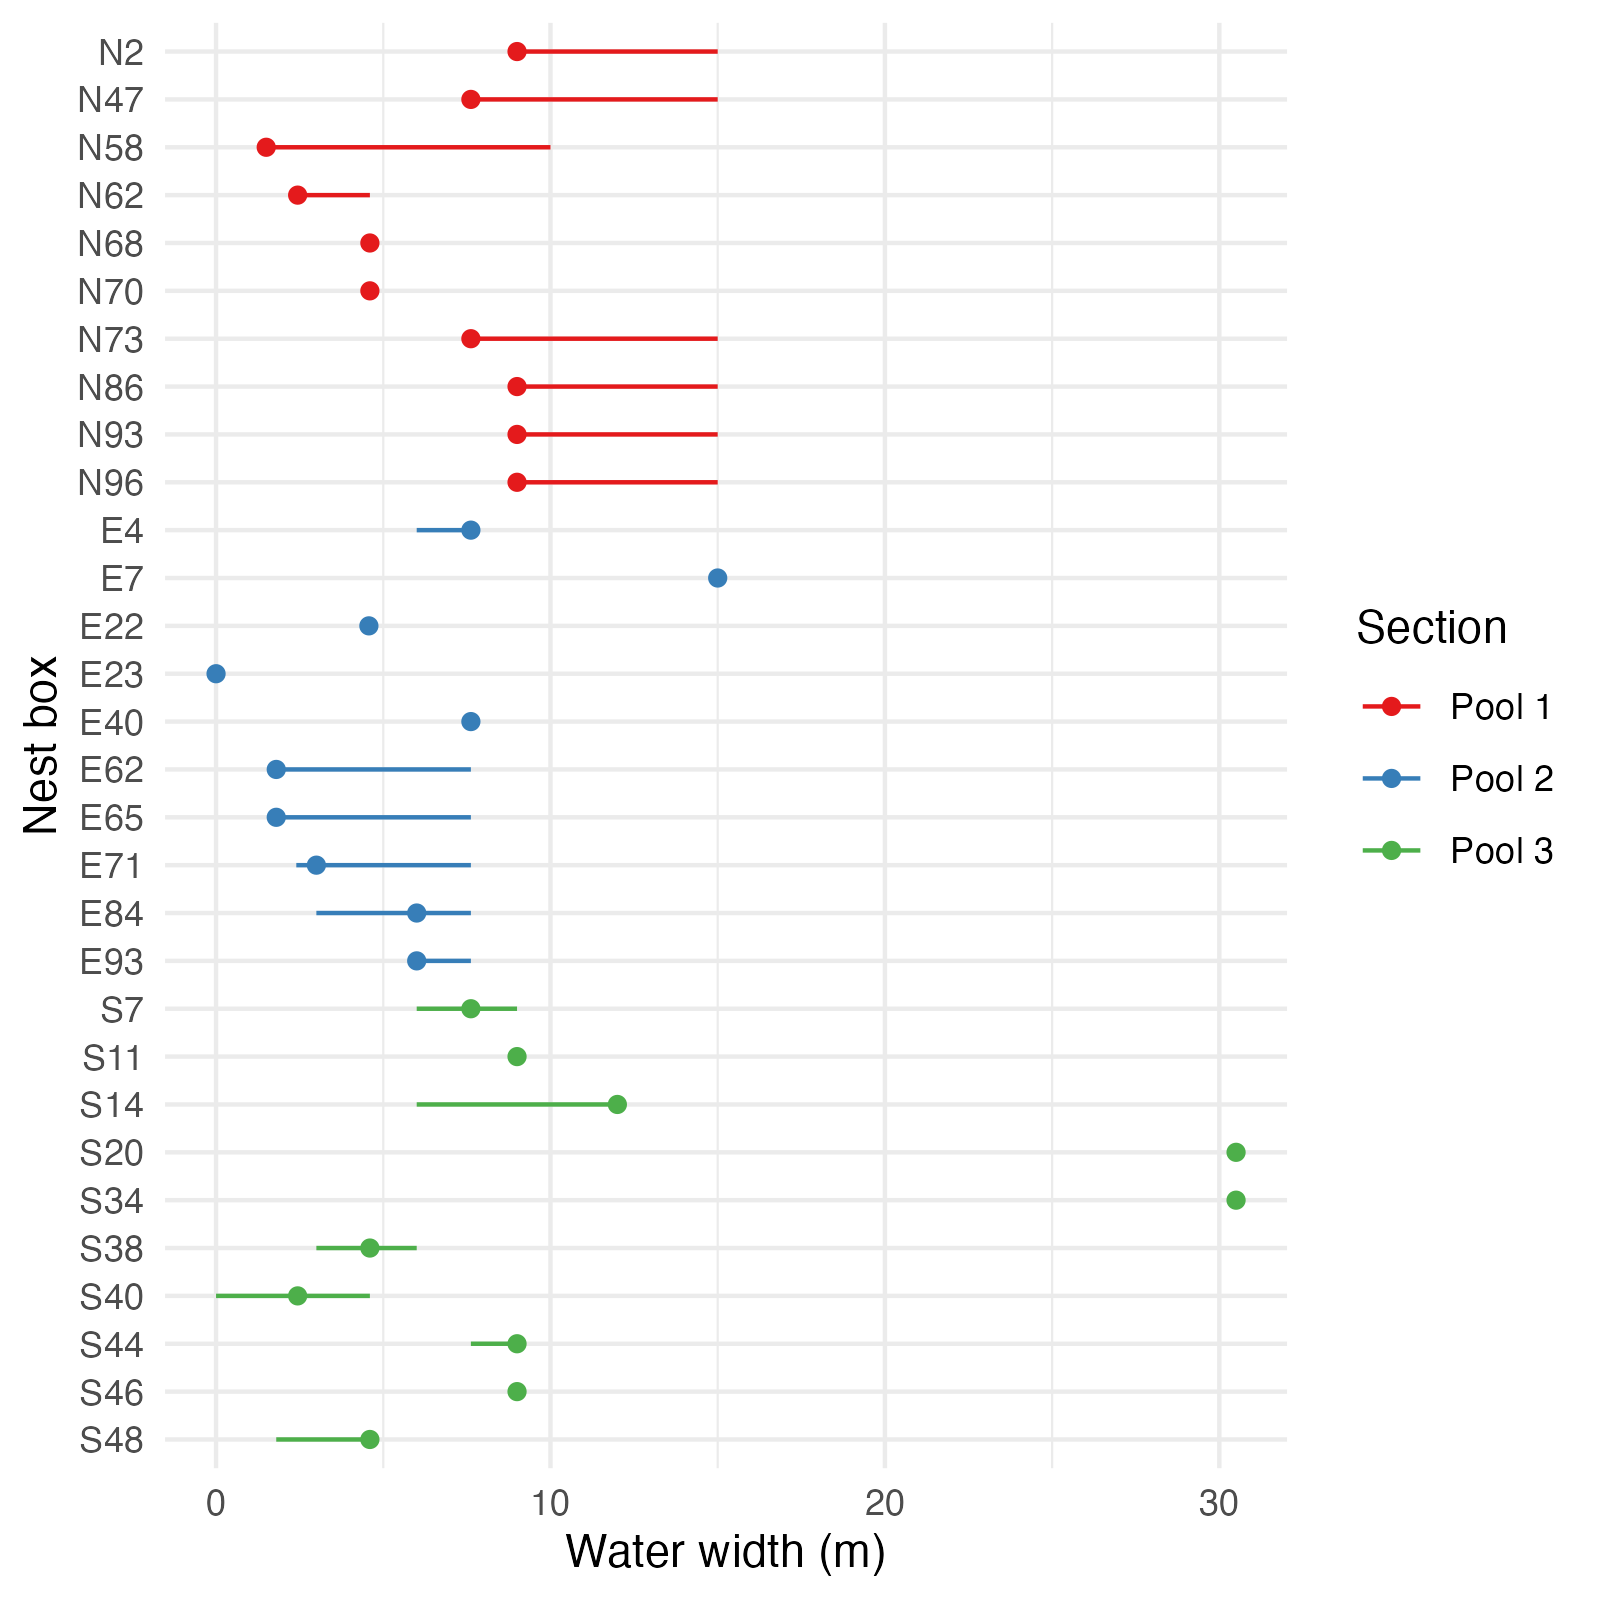
\includegraphics[width=\textwidth]{water_width_plot}
	\caption[Range and mode of water width measured for each nest box.]{Range and mode of water width measured weekly for each nest box during the study. Range is indicated by line segments. Mode is indicated by dots.}
	\label{fig:water_width_plot}
\end{figure}
\clearpage}


\afterpage{%
\begin{figure}[p!]
	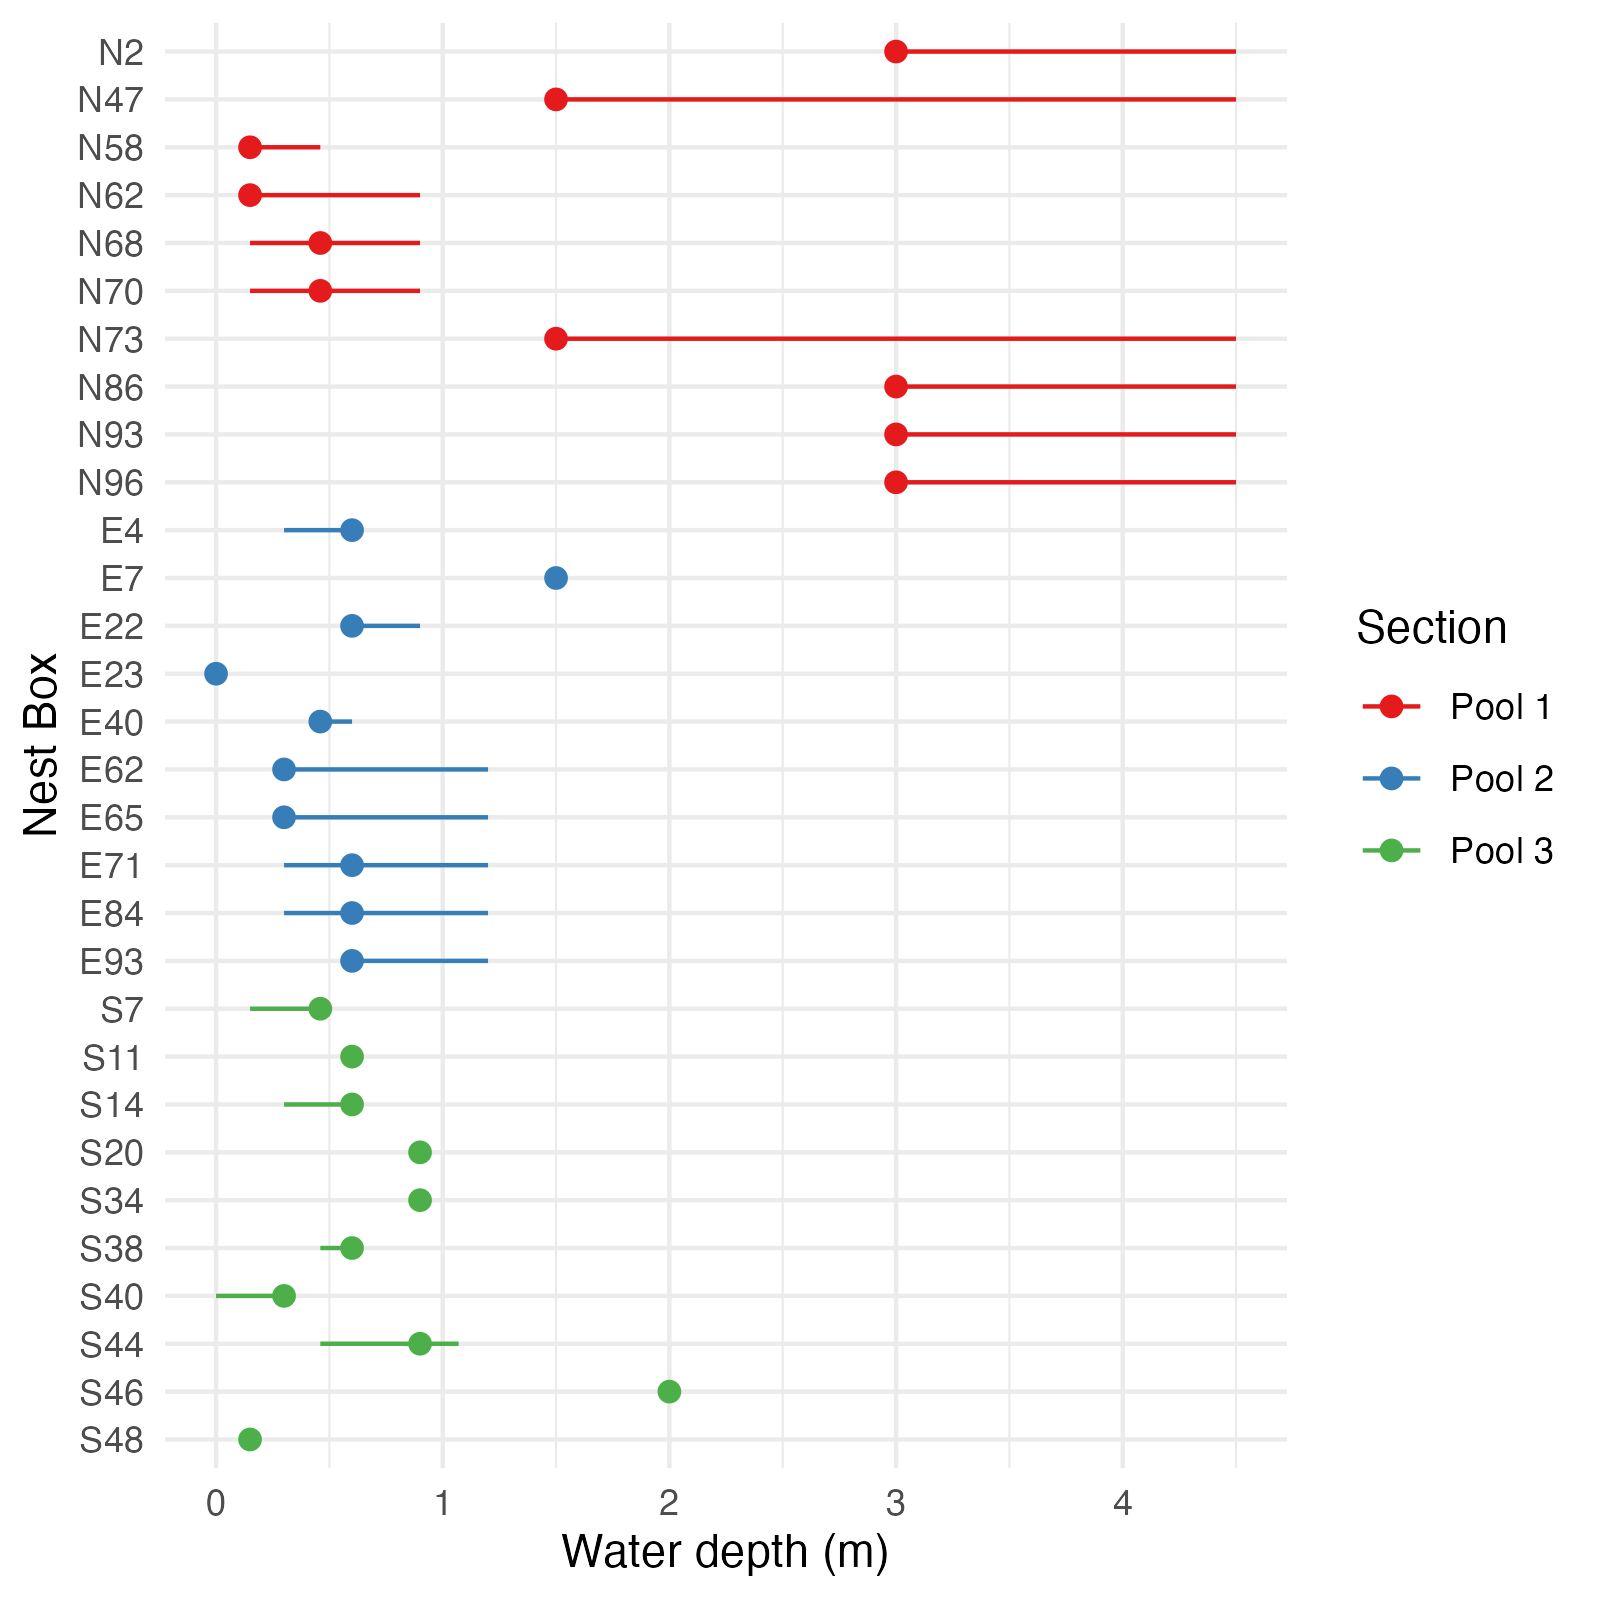
\includegraphics[width=\textwidth]{water_depth_plot}
	\caption[Range and mode of water depth measured for each nest box.]{Range and mode of water depth measured weekly for each nest box during the  study. Range is indicated by line segments. Mode is indicated by dots.}
	\label{fig:water_depth_plot}
\end{figure}
\clearpage}


Tree coverage differed significantly among the 3 pools ($F_{2,20} = 6.032, p < 0.009$; Table~\ref{tab:anova_coverage}; Figure~\ref{fig:tree_coverage_plot}). Pool~1 was significantly more open ($\overline{x} = 13{,}628$ \unit{\meter\squared}) compared to Pool~2 ($\overline{x} = 25{,}176$ \unit{\meter\squared}) and Pool~3 ($\overline{x} = 23{,}669$ \unit{\meter\squared}) (Table~\ref{tab:coverage_hsd_table} and Figure~\ref{fig:hsd_coverage_plot}, Appendix A), due to the proximity of the large and open areas of Pool~1 and Unit~A. 

\afterpage{%
%\begin{Spacing}{1}
\begin{table}
\addfontfeatures{Numbers=Monospaced}
\centering
\begin{threeparttable}
\caption[Analysis of variance results for amount of tree coverage]{Analysis of variance results for amount of tree coverage among the three pools in Duck Creek Conservation Area.}\label{tab:anova_coverage}
\noindent\begin{tabular}[l]{@{}lrrrrr@{}}
\toprule
Source of variation & $df$ & $SS$ & $MS$ & $F$ & $p$ \tabularnewline
\midrule
Pool & 2 & 381221000 & 190610500 & 6.032 & 0.00891 \tabularnewline
Residuals & 20 & 631951315 & 31597566 & & \tabularnewline
\bottomrule
\end{tabular}
\end{threeparttable}
\end{table}
%\end{Spacing}
\clearpage
}

\afterpage{%
\begin{figure}[p!]
	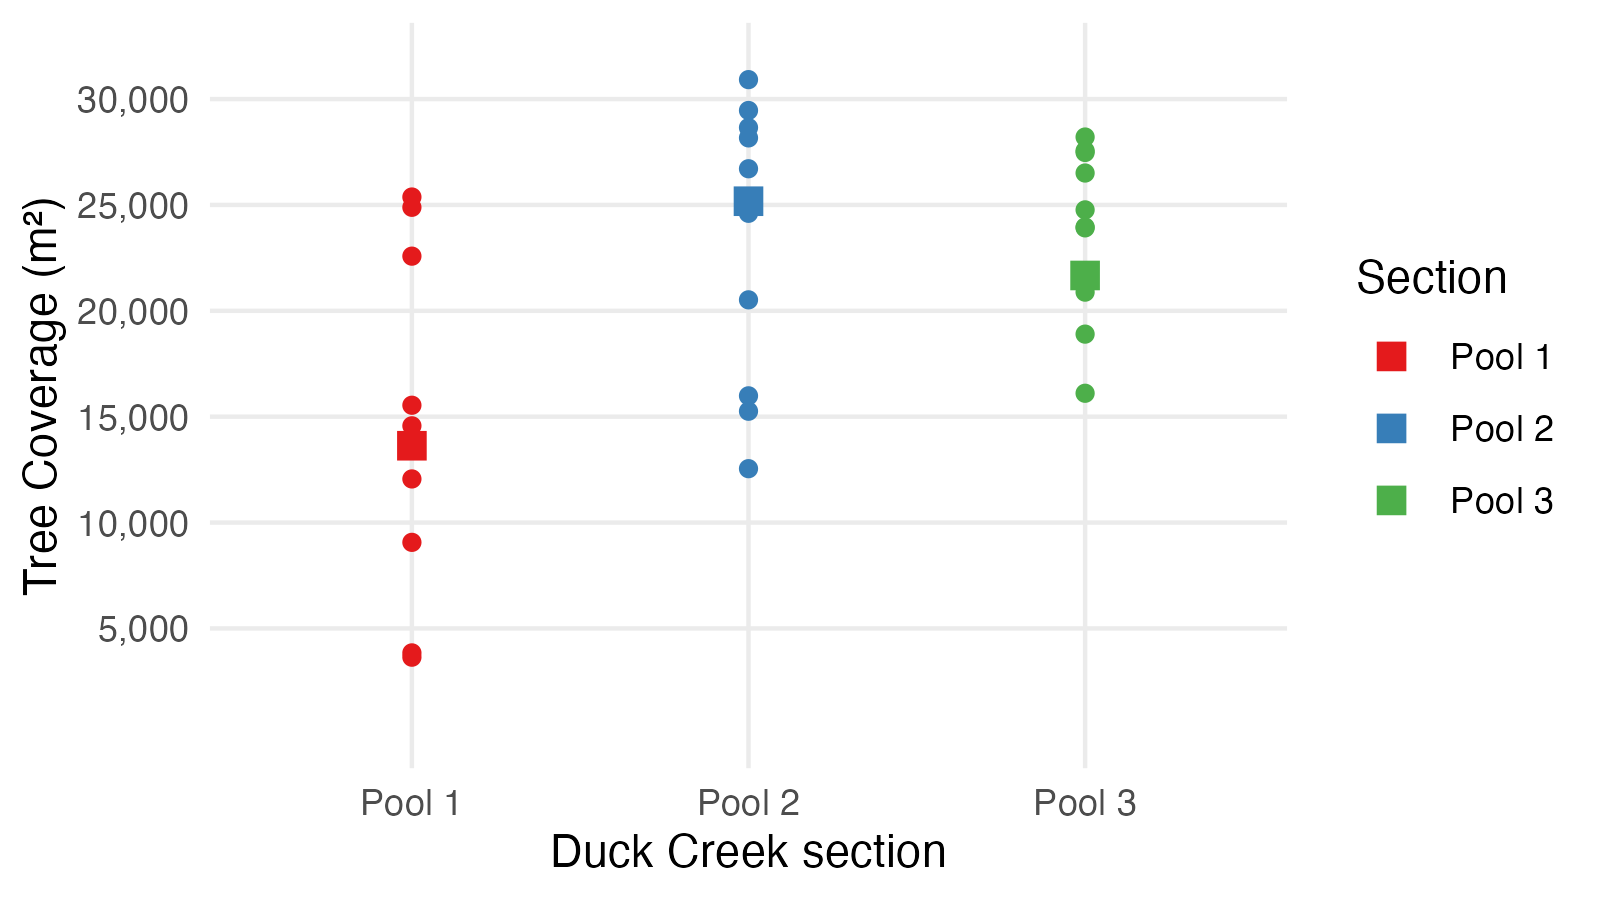
\includegraphics[width=\textwidth]{tree_coverage_plot}
	\caption[Range and mean of tree coverage]{Range and mean of tree coverage for each section. Dots indicate individual measurements. Triangle indicates mean coverage for each section.}
	\label{fig:tree_coverage_plot}
\end{figure}
\clearpage}


\section*{Nesting}

Nesting events occurred in 17 of the 30 nest boxes (56.7\%) during this study. A second, sequential nesting attempt occurred in 6 of the 17 boxes, for a total of 23 nests during the study period. The second attempts were treated as independent nesting events for analysis. 
Hooded Mergansers accounted for 9 nesting events and Wood Ducks accounted for the other 14 events (Tables~\ref{tab:hooded_merganser_data_table} and ~\ref{tab:wood_duck_data_table}).  Ten nesting events occurred in the Pool~2 in 7 boxes. Nine of the events were by Wood Ducks; only one was by Hooded Merganser. Nine nesting events occurred in the Pool~3 in 7 boxes. Five of the events were by from Hooded Mergansers and four were by Wood Ducks. Four nesting events occurred in Pool~1 in separate boxes. Three events were by Hooded Mergansers and only one by Wood Duck. %No nests were observed in natural cavities in the vicinity of these nest boxes.  

\afterpage{%
\begin{landscape}		
%\begin{Spacing}{1}
\begin{table}
\addfontfeatures{Numbers=Monospaced}
\centering
\begin{threeparttable}
\caption[Hooded Merganser data for boxes with nesting events]{Hooded Merganser data for boxes with nesting events. Original eggs were laid by the occupying hen. Dumped eggs were added by a different hen. Hatched, abandoned, and lost include original plus any dumped eggs. See Table~\ref{tab:raw_data_eggs} for detailed nesting results.} \label{tab:hooded_merganser_data_table}
\noindent\begin{tabular}[l]{@{}R{1.5cm}R{1.5cm}R{1.5cm}R{1.2cm}R{1.5cm}R{2.0cm}R{1cm}R{1.8cm}R{1.8cm}R{2.7cm}@{}}
\toprule
& \multicolumn{6}{c}{Number of Eggs} & \multicolumn{2}{c}{Water} & \tabularnewline
\cmidrule(rl){2-7} \cmidrule(rl){8-9}
Nest box & Original & Dumped & Total & Hatched & Abandoned & Lost & Depth (m) & Width (m) & Tree Cover (m²) \tabularnewline
\midrule
E40 & 11 & 0 & 11 & 11 & 0 & 0 & 0.46 & 7.62 & 29,461\tabularnewline
S34 & 9 & 0 & 9 & 0 & 9 & 0 & 0.9 & 30.5 & 18,899\tabularnewline
S34 & 9 & 0 & 9 & 0 & 9 & 0 & 0.9 & 30.5 & 18,899\tabularnewline
S7 & 2 & 10 & 12 & 11 & 1 & 0 & 0.46 & 7.62 & 16,106\tabularnewline
S11 & 10 & 0 & 10 & 10 & 0 & 0 & 0.6 & 9 & 27,559\tabularnewline
S44 & 11 & 2 & 13 & 11 & 2 & 0 & 0.9 & 9 & 27,478\tabularnewline
N93 & 20 & 2 & 22 & 18 & 2 & 2 & 4.5 & 15 & 3,642\tabularnewline
N2 & 16 & 0 & 16 & 16 & 0 & 0 & 4.5 & 15 & 12,060\tabularnewline
N47 & 8 & 0 & 8 & 8 & 0 & 0 & 1.5 & 7.62 & 25,374\tabularnewline\bottomrule
\end{tabular}
\end{threeparttable}
\end{table}
%\end{Spacing}
\end{landscape}
\clearpage
}



\afterpage{%
\begin{landscape}		
%\begin{Spacing}{1}
\begin{table}
\addfontfeatures{Numbers=Monospaced}
\centering
\begin{threeparttable}
\caption[Wood Duck data for boxes with nesting events]{Wood Duck data for boxes with nesting events. Original eggs were laid by the occupying hen. Dumped eggs were added by a different hen. Hatched, abandoned, and lost include original plus any dumped eggs. See Table~\ref{tab:raw_data_eggs} for detailed nesting results.} \label{tab:wood_duck_data_table}
\noindent\begin{tabular}[l]{@{}R{1.5cm}R{1.5cm}R{1.5cm}R{1.2cm}R{1.5cm}R{2.0cm}R{1cm}R{1.8cm}R{1.8cm}R{2.7cm}@{}}
\toprule
& \multicolumn{6}{c}{Number of Eggs} & \multicolumn{2}{c}{Water} & \tabularnewline
\cmidrule(rl){2-7} \cmidrule(rl){8-9}
Nest box & Original & Dumped & Total & Hatched & Abandoned & Lost & Depth (m) & Width (m) & Tree Cover (m²) \tabularnewline
\midrule
E62 & 10 & 3 & 13 & 10 & 3 & 0 & 0.3 & 1.8 & 28,166\tabularnewline
E62 & 8 & 5 & 13 & 12 & 0 & 1 & 0.3 & 2.4 & 28,166\tabularnewline
E65 & 17 & 1 & 17 & 16 & 0 & 1 & 0.3 & 3 & 24,605\tabularnewline
E93 & 9 & 0 & 9 & 9 & 0 & 0 & 0.9 & 6 & 20,518\tabularnewline
E93 & 2 & 0 & 2 & 0 & 0 & 2 & 1.2 & 7.62 & 20,518\tabularnewline
E4 & 14 & 0 & 14 & 0 & 6 & 8 & 0.6 & 7.62 & 30,918\tabularnewline
E7 & 9 & 1 & 10 & 9 & 1 & 0 & 1.5 & 15 & 15,985\tabularnewline
E22 & 8 & 4 & 12 & 8 & 4 & 0 & 0.6 & 4.57 & 26,709\tabularnewline
E22 & 14 & 0 & 14 & 0 & 0 & 14 & 0.9 & 4.57 & 26,709\tabularnewline
S20 & 13 & 6 & 19 & 13 & 6 & 0 & 0.9 & 30.5 & 20,882\tabularnewline
S20 & 17 & 4 & 21 & 15 & 4 & 2 & 0.9 & 30.5 & 20,882\tabularnewline
S7 & 13 & 3 & 16 & 13 & 1 & 2 & 0.46 & 9 & 16,106\tabularnewline
S14 & 19 & 2 & 21 & 13 & 1 & 7 & 0.6 & 12 & 28,207\tabularnewline
N70 & 2 & 4 & 6 & 2 & 4 & 0 & 0.15 & 4.6 & 13,436\tabularnewline\bottomrule
\end{tabular}
\end{threeparttable}
\end{table}
%\end{Spacing}
\end{landscape}
\clearpage
}



Nesting success was based on the number of hatched eggs, including dumped eggs. Hooded Merganser hatched \numrange[range-phrase = –]{0}{18}, with a mean of \num{8.3} eggs. Wood Duck hatched \numrange[range-phrase = –]{0}{16} eggs, with a mean of \num{9.3} eggs. The number of hatched eggs was not significantly different between species ($t = -0.388, p = 0.702$). A significant interaction effect for number of eggs hatched did occur between species and pool ($F_{2,18} = 5.96, p < 0.05$; Table~\ref{tab:anova_table}). Hooded Merganser hatched a total of 42 eggs in the Pool~1 in three events compared to 11 eggs in Pool~2  (1 event) and 32 eggs in Pool~3 (5 events, including 2 failed events; Table~\ref{tab:hooded_merganser_data_table}; Figure~\ref{fig:hatched_eggs_plot}). Wood Duck hatched 64 eggs in Pool~2 in 6 boxes (9 events, including 3 failed). %Three boxes were used for sequential events. The second attempts in boxes E22 and E93 both failed. 
Wood Duck hatched 54 eggs in Pool~3 across four events in three boxes. This species made only one attempt in Pool~1 and hatched just 2 eggs (Table~\ref{tab:wood_duck_data_table}; Figure~\ref{fig:hatched_eggs_plot}). 

\afterpage{%
%\begin{Spacing}{1}
\begin{table}
\addfontfeatures{Numbers=Monospaced}
\centering
\begin{threeparttable}
\caption[Analysis of variance results for number of hatched eggs by species and pool]{Analysis of variance results for number of hatched eggs by species and pool.}\label{tab:anova_table}
\noindent\begin{tabular}[l]{@{}lrrrrr@{}}
\toprule
Source of variation & $df$ & $SS$ & $MS$ & $F$ & $p$ \tabularnewline
\midrule
Species & 1 & 4.9 & 4.90 & 0.216 & 0.648 \tabularnewline
Pool & 2 & 37.4 & 18.71 & 0.824 & 0.455 \tabularnewline
Species * Section & 2 & 270.6 & 135.31 & 5.957 & 0.010 \tabularnewline
Residuals & 18 & 408.9 & 22.72 &  & \tabularnewline
\bottomrule
\end{tabular}
\end{threeparttable}
\end{table}
%\end{Spacing}
\clearpage
}

\afterpage{%
\begin{figure}[p!]
	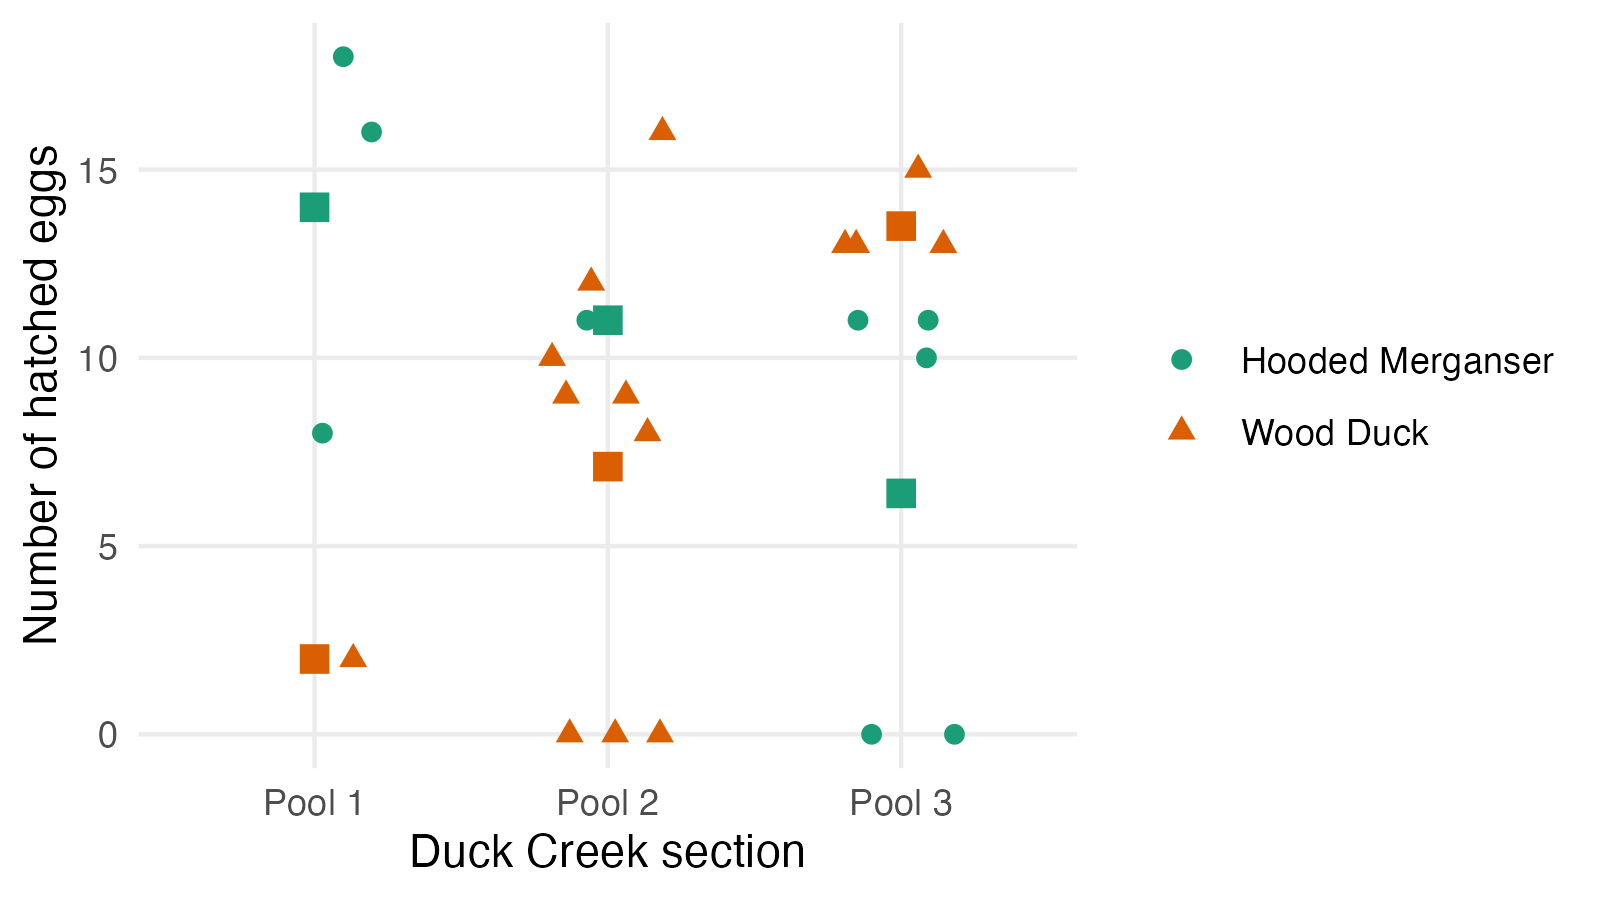
\includegraphics[width=\textwidth]{hatched_eggs_plot}
	\caption[Number of hatched eggs per nest box by pool]{Number of hatched eggs per nest box by pool. Green circles represent individual values for Hooded Merganser. Orange triangles represent individual values for Wood Duck. Green and orange squares represent mean number of eggs hatched in each pool for Hooded Merganser and Wood Duck, respectively. }
	\label{fig:hatched_eggs_plot}
\end{figure}
\clearpage}
 

Dump nesting was observed in 3 of 9 Hooded Merganser nests (Figure~\ref{fig:dumped_eggs_plot}). Egg dumping in Hooded Merganser nests occurred in nest boxes N93, S7, and S44, with 2, 2, and 10 eggs, respectively. These are the only three Hooded Merganser nests that did not have 100\% hatching success (Table~\ref{tab:hooded_merganser_data_table}). The most extreme dump nesting event for a Hooded Merganser hen was in nest box S7. The original hen laid only 2 eggs. An additional 10 eggs were added by Wood Duck. Only one Hooded Merganser egg hatched. The second was abandoned. All 10 Wood Duck eggs hatched (Table~\ref{tab:raw_data_eggs}, Appendix A). This was the only observed event where Wood Duck dump-nested in a Hooded Merganser nest.

In comparison, dump nesting occurred in 10 of 14 Wood Duck nests. The number of eggs dumped in Wood Duck nests ranged from 1–6, with a mean of 3.3 eggs. Only boxes E65, S20 attempt 2, and S14 saw fewer eggs hatched than those originally laid by the Wood Duck hen. Box E65 was the only observed instance of a Hooded Merganser egg being nest-dumped in a Wood Duck nest. For most cases, the number of eggs hatch in a nest with known dump-nesting, the number of eggs hatched matched the number of eggs laid originally by the Wood Duck hen.


\afterpage{%
\begin{figure}[p!]
	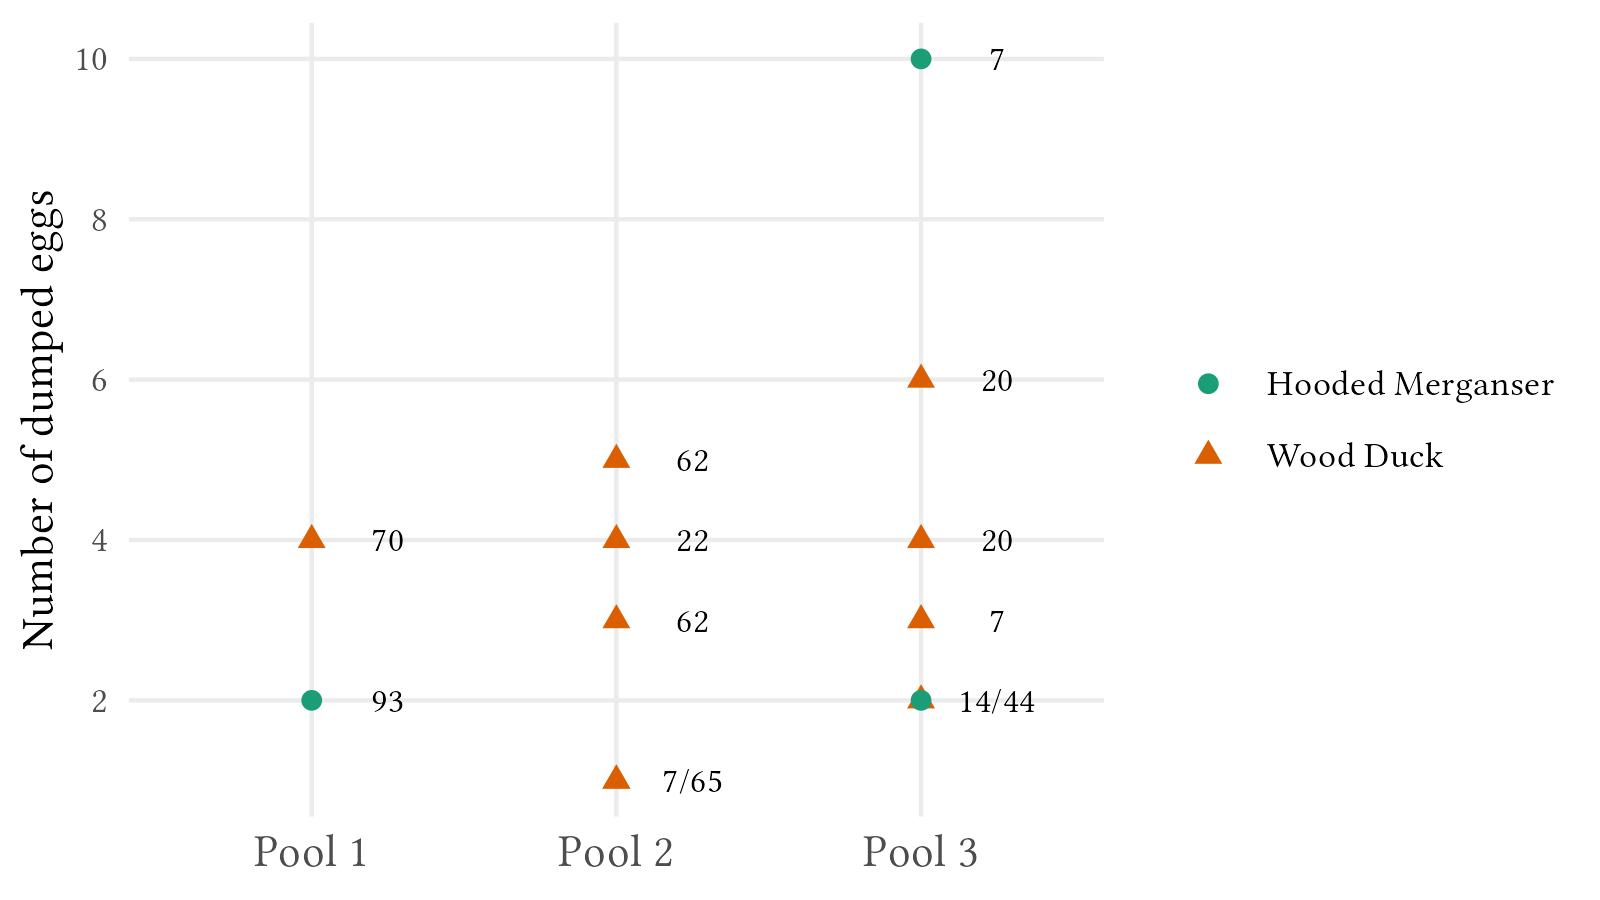
\includegraphics[width = \textwidth]{dumped_eggs_plot}
	\caption[Nest boxes with evidence of egg dumping]
	{Nest boxes with evidence of egg dumping for each pool of the study. Green circles indicate boxes with Hooded Merganser as the host species. Orange triangles indicate boxes with Wood Duck as the host species. Boxes N7 and N65 both had one egg dumped. Boxes S14 and S14 both had two eggs dumped. Box E62 had sequential nesting events, both by Wood Duck. Box S7 had sequential nesting events, first by Hooded Merganser followed by Wood Duck.}
	\label{fig:dumped_eggs_plot}
\end{figure}
\clearpage}
 


The relationship among hatching, water width and depth, and tree coverage was revealed by the \textsc{nmds} analysis (Figures~\ref{fig:nmds_plot_axes12} and~\ref{fig:nmds_plot_axes23}).  Both species had successful hatching for most nests (Figures~\ref{fig:nmds_plot_axes12} and~\ref{fig:hatched_eggs_plot}). Three Hooded Merganser nests were on the west side of the North section, which tended to have deeper water (Figures~\ref{fig:water_depth_plot} and~\ref{fig:nmds_plot_axes23}). Hooded Merganser had their highest number of eggs hatched in Pool~1 with nest boxes N2 and N93 (Figures~\ref{fig:hatched_eggs_plot} and~\ref{fig:nmds_plot_axes12}) although fewer eggs were hatched in nest box N47. Hooded Merganser did have success in Pool~2 and Pool~3. Two failed nests for Hooded Merganser were in Pool~3, both in box S34. 

\afterpage{%
\begin{figure}[p!]
	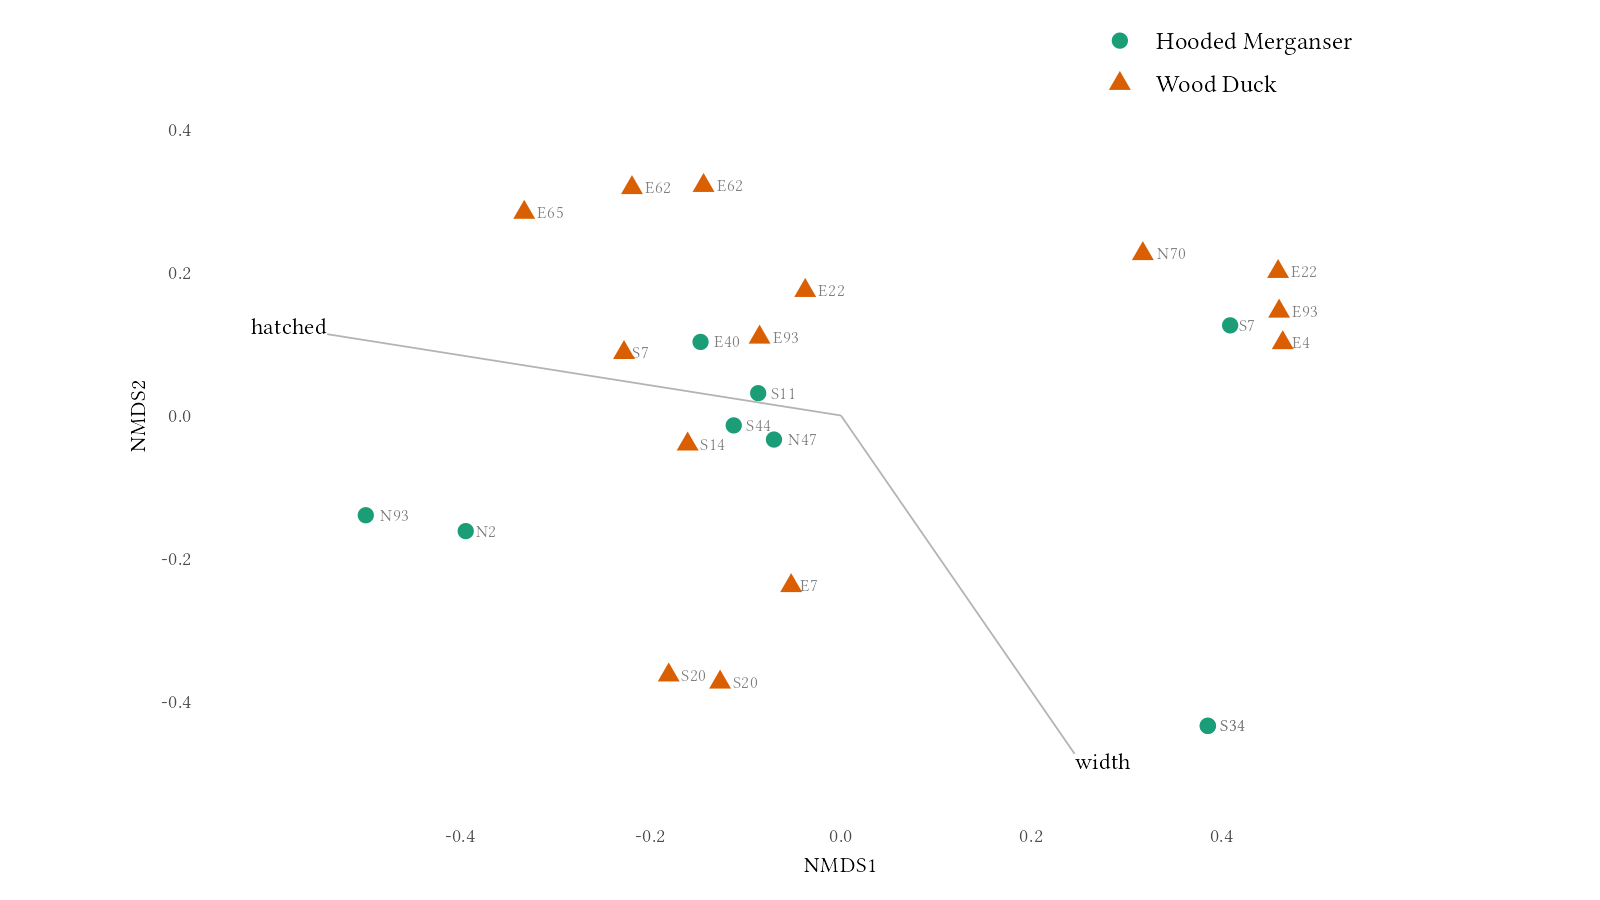
\includegraphics[width=\textwidth]{nmds_plot_axes12}
	\caption[N\textsc{mds} plot of axes 1 and 2]{Non-metric multidimensional analysis plot of axes 1 and 2. Green circles indicate nest boxes with Hooded Merganser as the original species. Orange triangles indicate nest boxes with Wood Duck as the original species. Light gray numbers show box~\textsc{id} numbers. N = Pool~1; E = Pool~2, S = Pool~3. Hatched and width variables provided the greatest rank-order separation on axis~1 and axis~2, respectively. Boxes to the left of the plot had greater numbers of hatched eggs. Boxes toward the lower half of the plot were associated with wider water. Stress = 0.023.}
	\label{fig:nmds_plot_axes12}
\end{figure}
\clearpage}
 

\afterpage{%
\begin{figure}[p!]
	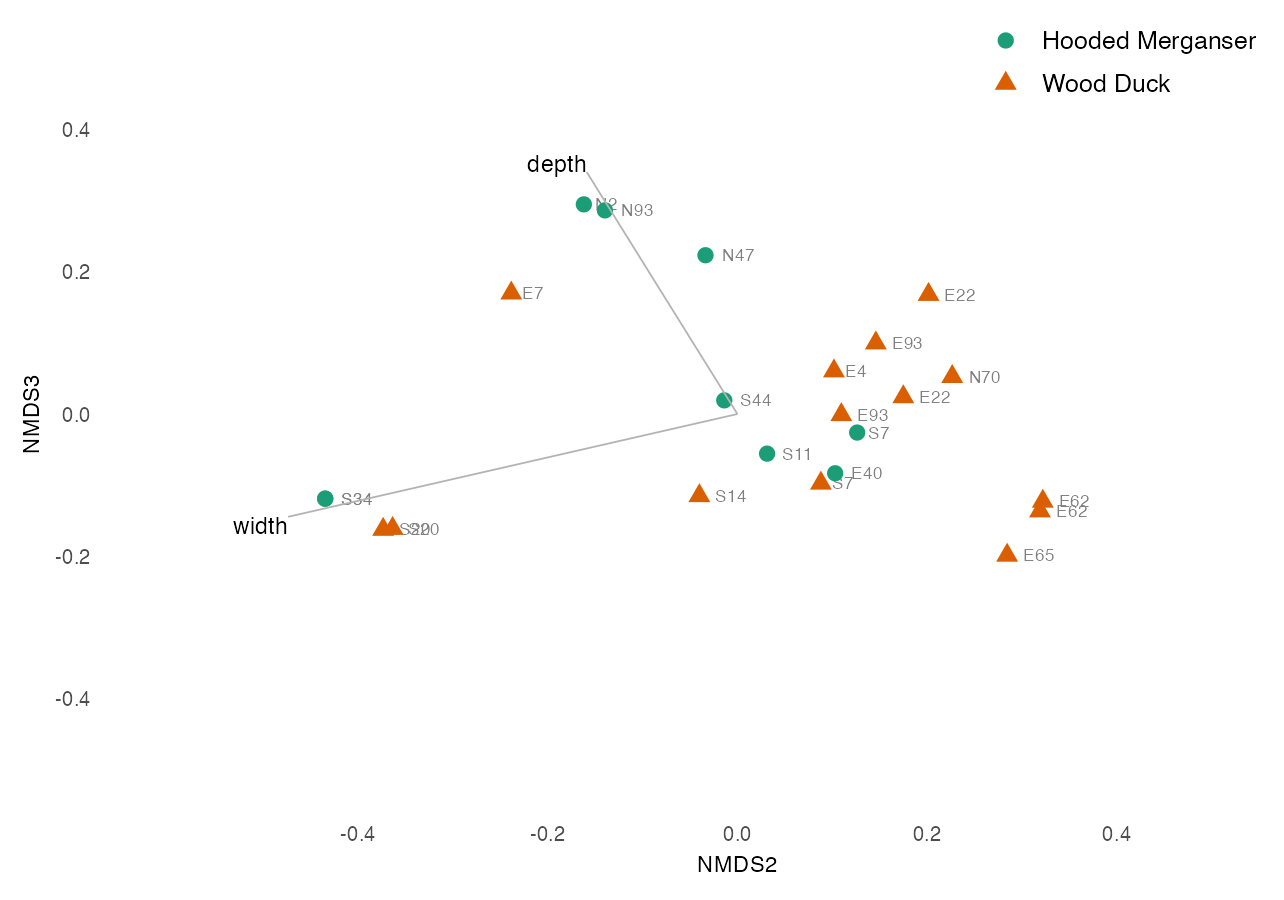
\includegraphics[width=\textwidth]{nmds_plot_axes23}
	\caption[N\textsc{mds} plot of axes 2 and 3]{N\textsc{mds} plot of axes 2 and 3.  Stress = 0.023.}
	\label{fig:nmds_plot_axes23}
\end{figure}
\clearpage}
 

Wood Duck nested mostly along the relatively shallow, narrow ditches (Figure~\ref{fig:nmds_plot_axes12}) of Pool~2 and Pool~3. They established only one nest on the east side of Pool~1 where the ditch is relatively shallow and narrow. Wood Duck did have two sequential nesting attempts in Pool~3 in the nest box S20, which is located along a broad, shallow pool. Wood Duck had two failed attempts in Pool~3 in nest boxes E4 and E93 (Figures~\ref{fig:hatched_eggs_plot} and~\ref{fig:nmds_plot_axes12}). %N\textsc{mds} stress was \num{0.023}, indicating a very good fit between the data and ordination results.


